\section{Einführung}
\subsection{Literatur}
\begin{enumerate}
  \item \textsc{Kerson Huang}. \emph{Statistical Mechanics}, J. Wiley.
  \item \textsc{L.E. Reichl}. \emph{A Modern Course in Statistical Physics}, Arnold Publ.
  \item \textsc{G. A. Adam, O. Hitmair}. \emph{Wärmetheorie}, Vieweg.
\end{enumerate}
\subsection{Stellung der statistischen Physik}
\begin{itemize}
  \item Untersucht werden Systeme mit mikroskopischen (sehr) \emph{vielen} \emph{Freiheitsgraden} \\ 
  		(Vielteilchensystem)
  \item Makroskopische Beschreibung durch \emph{wenige Parameter}
\end{itemize}
\begin{figure}[H]
\begin{center}
  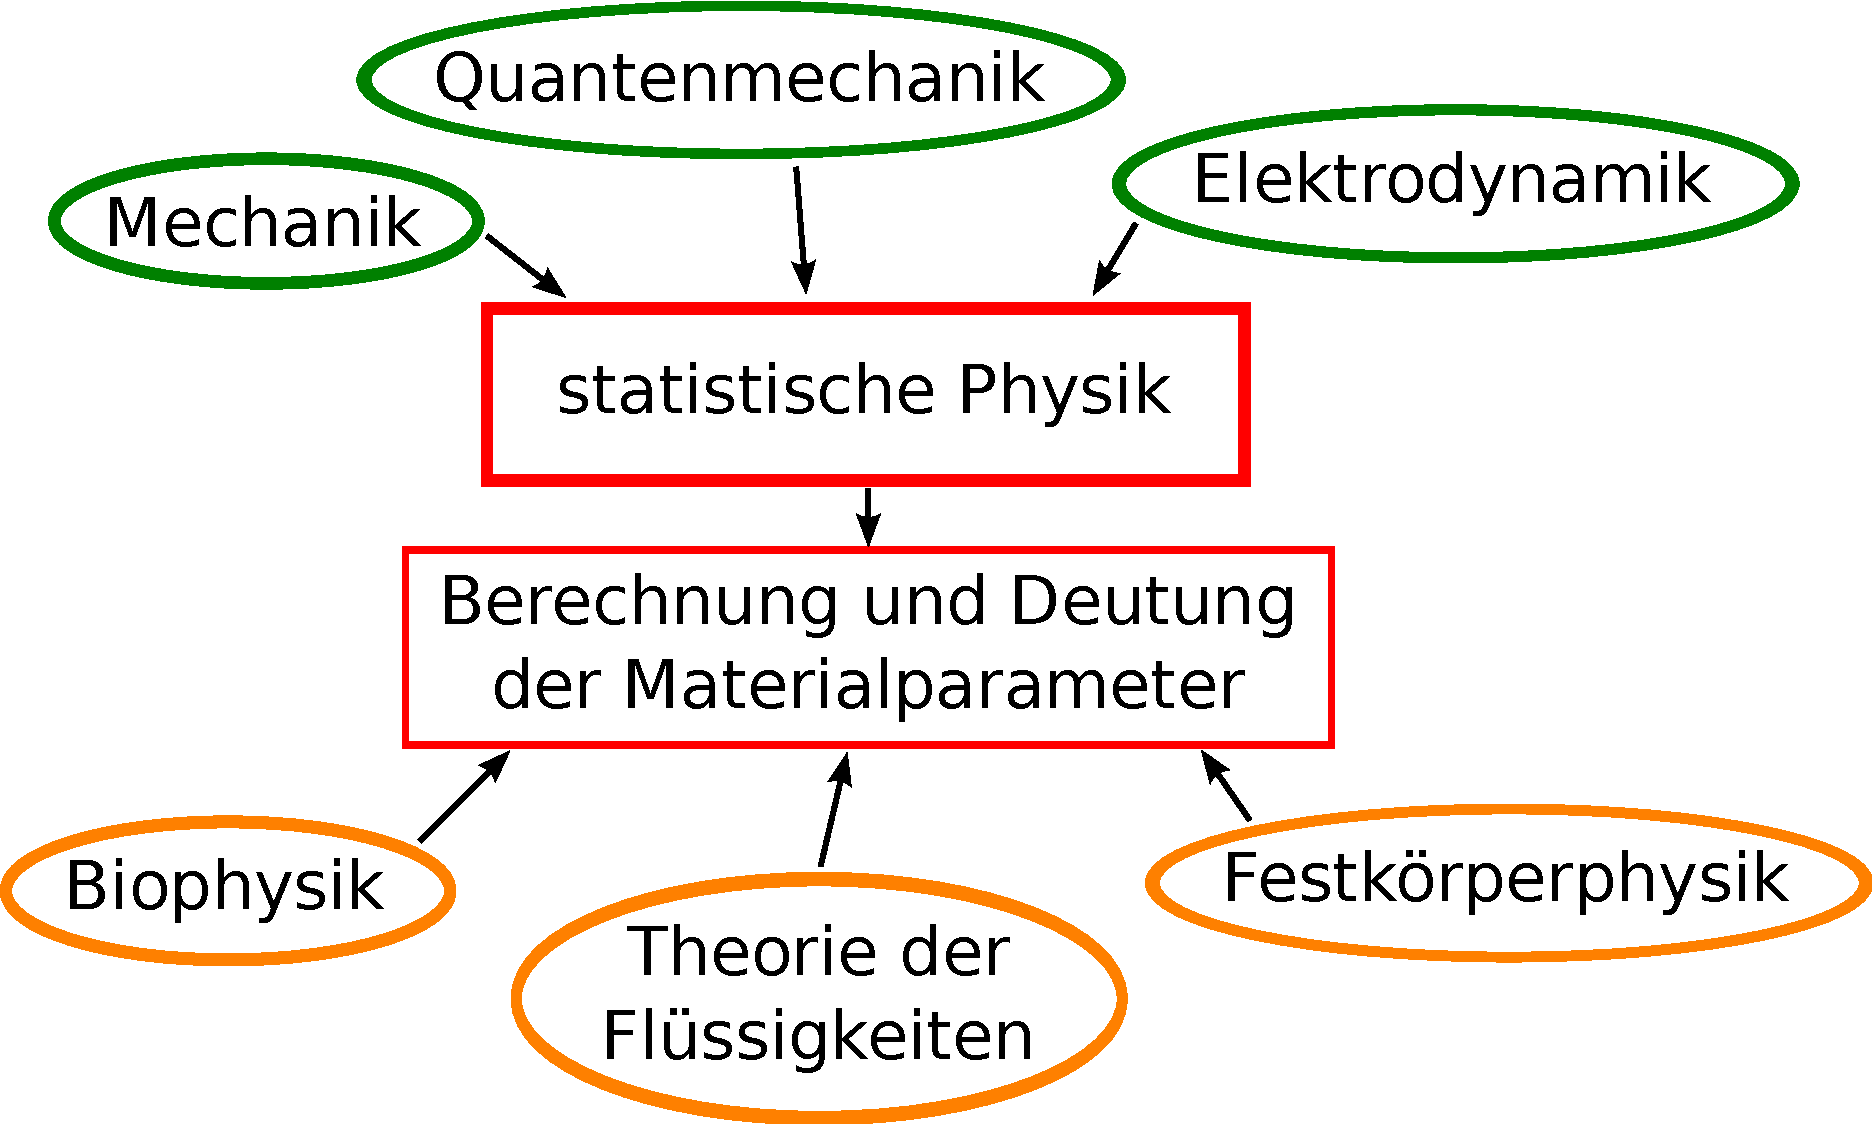
\includegraphics[width=\textwidth]{../img/dependencies.pdf}
  \caption{Stellung der statistischen Physik.}
  \label{img:position_statphys}
\end{center}
\end{figure}